\chapter{Evaluation}
\label{ch:evaluation}
This chapter gives an overview of the results and how the benchmark is set up.
The used tools and relevant metrics are introduced for the respective technologies.
Further the evaluation criteria is given and the summary of the results is discussed.

\section{Setup and Methodology}
\label{sec:evaluation_setup}
In order to evaluate the framework's performance, a use-case based approach with two real-world applications is chosen.
In the course of this thesis following two applications are used for the experiments:\\
The first application is designed to mainly deal with I/O operations, based on IoT data, is described in section \ref{sec:iot_application}.
To get the SMACK stack close to its limit the load generator and stress test tool introduced in section \ref{sec:load_generator} are used.\\
The second application used to evaluate the auto-scaling framework is introduced in section \ref{sec:computation_application}.
As the scenario here is fundamentally different, it is a good indicator whether the framework is able to correctly monitor and scale the stack or not.
Most of the computation power is needed in Apache Spark, which the framework should detect and assign the most resources to this service.\\


\subsection{Load Generator and Stress Test}
\label{sec:load_generator}
To be able to test the application described in Section~\ref{sec:iot_application} a load generator was designed.
The tool has two modes - either pre-recorded real life IoT sensor data, or random data, can be send to the cluster.\\
In principle the tool just sends lots of HTTP requests to the server, while the JSON data is not interpreted and only treated as plain string.
In the random mode, only the timestamp of the entries is randomized, as it is enough to cause unique entries in the Cassandra database.\\

The mode with real data requires the data to be provided in a specific format.
In the source code there is a tool for formatting JSON files into the proper format to be used further.
As one HTTP request contains a whole sensor data JSON entry of a device, it is of favor, to concatenate the entries into a single line.
This reduces the CPU load, as the parsing can be omitted and one line equals one request.
With the help of the provided tool, text files with multiple JSON entries can be joined together to one larger text file containing single-line entries.
The advantage of using a few large files over multiple smaller files is that the disk time can be reduced dramatically during reading, which causes higher throughput.\\
In addition the milliseconds of the timestamp of each entry is randomize to avoid duplicates in the database.
This has to be done at runtime and cannot be pre computed in advance.\\

The contribution of this thesis to the tool is the optimization of the data format, as well as integrating randomization to achieve unique database entries even when the tools runs in parallel with the same input data.\\

To be able to orchestrate multiple clients at once, the load generator is deployed into a Docker image.
AWS provides a service called \textit{Elastic Cloud Computing Container Service (ECS)}.
It allows the user to easily deploy, manage and scale Docker containers in a managed cluster.\\
There are a few advantages of using this service: It is as easy as clicking on "scale" to instantiate more containers and distribute them equally across the cluster.
Amazon allows the user to configure how the containers are distributed, for example place each container on a different node to provide equal stress among the cluster, or to pack everything on one node until its working capacity is full.
In addition many other AWS services are integrated, like Elastic Load Balancing, etc.
An important feature is the command line API, which helps to automatically launch and stop instances in the cluster.\\

In Figure~\ref{fig:aws_ecs} the service is illustrated and shows the individual components.
The unit of execution is always a Docker image, which can be pulled from any available container registry.
It is possible to use mainstream platforms like Docker Hub, host it at Amazon or provide a self-hosted solution.\\
Next, ECS requires the user to create a so called task definition, which is basically a JSON file which contains parameters like the container name, open ports, CPU and memory resources, mappings, etc.
There is also a web interface to easily create a task without having to write JSON.
Now it is possible to launch and stop tasks with AWS ECS doing all the work of distributing and running the container images with the correct parameters across the cluster.
Further a service can be created which defines different scheduling options and can be used to maintain a desired number of container instances or tasks executing simultaneously.\\

All the containers run inside a Virtual Private Cloud (VPC), which helps to easily integrate the cluster in existing solutions.
Amazon also provides the option to create a dedicated VPC for the ECS cluster without any configuration effort.
The cluster itself is a logical grouping of AWS Elastic Cloud Computing (EC2) instances, which can run in different Availability Zones (AZ).
This allows the user to logically distribute clusters and reduce network latency.
To be able to execute tasks and monitor the EC2 instances used for the ECS service, a container agent is running on each node and provides the AWS ECS controller with information and allows autonomous interaction.\\

To be able to run the load generator in the cloud by using AWS ECS, the creation of a Docker image, containing all necessary sensor data, was performed as part of this thesis.
Additionally the required task definition was created and a simple bash script to launch an arbitrary number of container instances in the cluster.


\begin{figure}[!htbp]
  \centering
  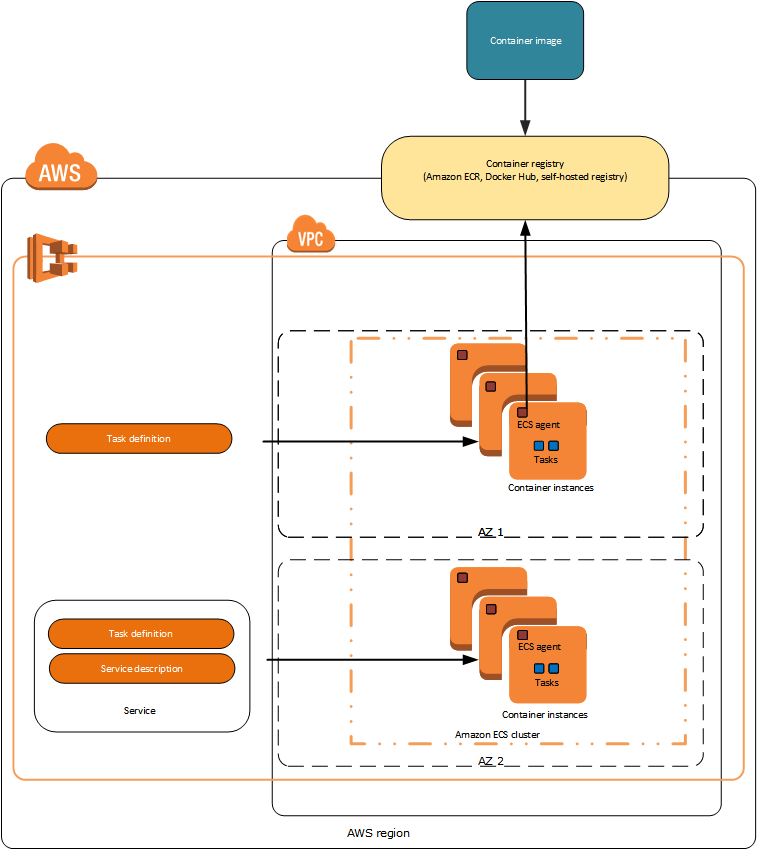
\includegraphics[keepaspectratio=true,scale=0.75]{img/aws_ecs}
    \caption{Overview of Amazon WebServices Elastic Cloud Computing Container Service \cite{aws}}
  \label{fig:aws_ecs}
\end{figure}


\subsection{Sensor Data Overview}
\label{sec:sensor-data}
The data used for the IoT application comes from sensors in elevators which were used during the HackZurich.
Mobile phones were placed inside the elevators and used to gather various information about like acceleration, noise, light, etc.\\
In this section the available data is listed and explained in roughly.

\begin{itemize}
    \item Accelerometer\\
          "It is a measurement of acceleration along the three spatial axes at a moment of time" \cite{sensor-data}.
    \item Gyrometer\\
          This gives information about the device rotation rate.
    \item Magnetometer\\
          Gives information about the measured magnetic field surrounding the device. The unit is microteslas.
    \item DeviceMotion\\
          "The data represents measurements of the attitude, rotation rate, and acceleration of a device" \cite{sensor-data}.
    \item Barometer\\
          Indicates the relative changes of altitude.
    \item BatteryLevel\\
          Gives information about the remaining battery of the device.
    \item Microphone\\
          Represents the recorded noise in dB.
    \item Light\\
          The ambient sensor is used to determine how bright the light is.
    \item Beacon\\
          Any beacon recorded during the monitoring is represented by this class.
\end{itemize}

\begin{code}
\begin{minted}[frame=single,framesep=10pt,fontsize=\scriptsize,linenos]{json}
[
   {
      "z":-1.003677368164062,
      "x":-0.0066986083984375,
      "y":-0.036865234375,
      "date":"2016-09-05T14:49:18.413+02:00",
      "type":"Accelerometer"
   },
   {
      "z":-0.003133475338587232,
      "x":-0.06178427202540229,
      "y":0.07116925170684153,
      "date":"2016-09-03T08:40:17.552+02:00",
      "type":"Gyro"
   },
   {
      "z":-645.7014770507812,
      "x":-19.19688415527344,
      "y":140.535400390625,
      "date":"2016-09-05T14:50:23.371+02:00",
      "type":"Magnetometer"
   },
   {
      "attitude":{
         "quaternion":{
            "x":0.0180332360021854,
            "w":0.9998316704300516,
            "y":-0.003365478874680562,
            "z":-0.0003267357948271106
         },
         "rotationMatrix":{
            "m13":0.006718040909618139,
            "m12":-0.0007747425115667284,
            "m33":0.9993269443511963,
            "m32":-0.0360582023859024,
            "m31":-0.006741608958691359,
            "m21":0.0005319805932231247,
            "m11":0.9999771118164062,
            "m22":0.9993494153022766,
            "m23":0.03606259822845459
         },
         "pitch":-0.006722463864462229,
         "yaw":-0.000722464864462227,
         "roll":-0.001732463864562228
      },
      "date":"2016-09-05T14:49:26.286+02:00",
      "type":"DeviceMotion"
   },
   {
      "relativeAltitude":0,
      "pressure":95.66769409179688,
      "date":"2016-09-05T14:50:26.300+02:00",
      "type":"Barometer"
   },
   {
      "type":"Battery",
      "date":"2016-09-05T14:49:18.413+02:00",
      "batteryLevel":"1.0",
      "batteryState":"Full"
   },
   {
      "peakPower":-24.93737,
      "averagePower":-31.9056,
      "date":"2016-09-05T14:50:23.736+02:00",
      "type":"Microphone"
   },
   {
      "type":"Light",
      "date":"2016-09-05T14:49:18.413+02:00",
      "brightnes":"0.3414323"
   },
   {
      "beacons":[
         {
            "accuracy":4.084238652674522,
            "id":"F7826DA6-4FA2-4E98-8024-BC5B71E0893E",
            "major":59314,
            "rssi":-88,
            "minor":13391
         },
         {
            "accuracy":4.641588833612778,
            "id":"F7826DA6-4FA2-4E98-8024-BC5B71E0893E",
            "major":60085,
            "rssi":-89,
            "minor":55763
         }
      ],
      "date":"2016-09-13T10:04:04.034+02:00",
      "type":"Beacon"
   }
]
\end{minted}
\captionof{listing}{Sensor Data Content Example \cite{sensor-data}}
\end{code}



More detailed information can be found in the hackzurich-sensordata-ios repository \cite{sensor-data-repo}.


\subsection{Experiment Setup}
The goal of the experiment is to find out how well the scaling tool impacts the performance of the SMACK stack.
This section describes the experiment setup and which steps are taken to collect evaluation data.

\subsubsection{IoT Application}
In case of the IoT-application the following setup is chosen, which is also reflected by the architecture illustrated in Figure~\ref{fig:overall_view}:

\begin{enumerate}
\item Launch the REST Monitor.
\item Launch the DC/OS cluster.
\item Deploy the SMACK stack.
\item Launch the JMX Extraction tool.
\item Deploy the IoT application.
\item Instantiate the ECS Load Generator. \label{enum:load_generator_start}
\item Slowly increase the load by adding Docker container instances to ECS.\\
      Slowly means five new containers each minute until 50 instances are up to give the application and the SMACK stack time for warm-up.
      Then two containers per minute are launched until 70 containers are running.
      After that, one container per minute is added.
\item Evaluate the extracted metrics to see how much data the single services can handle until the stack crashes.\\
      Whether the stack is still healthy or not is determined by looking at the DC/OS health status of each service.
      In addition the Akka application provides a web interface with simple statistics which will be unavailable once the service crashes.
\item Stop the ECS Load Generator. \label{enum:load_generator_stop}
\item Restart / redeploy unhealthy services.
\item Launch the Scaling Tool.
\item Perform steps \ref{enum:load_generator_start} to \ref{enum:load_generator_stop}.
\end{enumerate}

There are two runs which are almost identical.\\
In the first run, the stack is unsupervised and no resource re-distribution is performed.
This gives a baseline of how well the stack and the application perform in a default setup.
After the stack crashed all extracted metrics are stored in the REST Monitor which can be then used to determine 1) when the stack or one component crashed exactly and 2) how much data could be handled (total MB/s), as well as other metrics.
Additionally the information about the performance of each service is stored and can be evaluated.\\
In the second run the Scaling tool is launched, analyzing the stack and - if necessary - scaling services up or down.
Again, after the stack crashes under the heavy input of the load generator, the metrics stored in the REST Monitor are analyzed.\\

As there is now statistical data available of both runs, the conclusion of whether the tool worked as expected or not can be made.
It is expected that the ingestion part of the SMACK stack, which is Akka and Kafka, will crash first in this scenario, as the application is mainly IO-bound.\\

The configuration of Kafka, Cassandra and is set to the defaults used by DC/OS, while Akka is deployed within the custom application, which therefore needs a custom configuration.
This is shown in Source~Code~\ref{code:akka_iot_config}, which serves as input for the Marathon framework to deploy the application.

\begin{code}
\begin{minted}[frame=single,framesep=10pt,fontsize=\scriptsize,linenos]{json}
{
  "id": "sensor-ingestion",
  "instances": 1,
  "cpus":1,
  "mem":1048,
  "disk": 100,
  "container":{
    "docker":{
      "forcePullImage":true,
      "image":"bwedenik/sensor-ingestion",
      "network":"HOST",
      "privileged": false
    },
    "type":"DOCKER"
  },
  "labels":{
    "HAPROXY_GROUP":"external",
    "HAPROXY_0_PORT": "8083"
  },
  "portDefinitions": [
    {
      "port": 10099,
      "protocol": "tcp",
      "labels": {}
    },
    {
      "port": 10100,
      "protocol": "tcp",
      "labels": {}
    }
  ],
  "healthChecks": [
    {
      "protocol": "TCP",
      "path": "/hello",
      "portIndex": 0,
      "gracePeriodSeconds": 300,
      "intervalSeconds": 60,
      "timeoutSeconds": 15,
      "maxConsecutiveFailures": 3,
      "ignoreHttp1xx": false
    }
  ]
}
\end{minted}
\captionof{listing}{Marathon Configuration for Akka Sensor Ingestion Application}
\label{code:akka_iot_config}
\end{code}

The Spark driver for \textit{KafkaToCassandra}, which is the number crunching job to parse the incoming data and write it into the database, is configured with the following parameters:\\
\verb|spark.cores.max=2 --driver-memory 8G|\\
\verb|spark.driver.cores=2 spark.executor.cores=2 --executor-memory 4G|\\

\begin{minipage}{\linewidth}
\begin{code}
\begin{minted}[frame=single,framesep=10pt,fontsize=\scriptsize,linenos]{bash}
spark.executor.extraJavaOptions=-Dcom.sun.management.jmxremote=true \
 -Dcom.sun.management.jmxremote.port=8092 -Dcom.sun.management.jmxremote.ssl=false \
 -Dcom.sun.management.jmxremote.authenticate=false
spark.driver.extraJavaOptions=-Dcom.sun.management.jmxremote=true \
 -Dcom.sun.management.jmxremote.port=8092 -Dcom.sun.management.jmxremote.ssl=false \
 -Dcom.sun.management.jmxremote.authenticate=false
\end{minted}
\captionof{listing}{Spark JMX Deployment Configuration}
\label{code:spark_jmx_config}
\end{code}
\end{minipage}

Further, to be able to extract JMX values from Spark, the configuration shown in Source~Code~\ref{code:spark_jmx_config} is required when deploying the driver.


\subsubsection{Acceleration Prediction Application}
The scenario of running this application in the SMACK stack is very similar to the previous one:

\begin{enumerate}
\item Launch the REST Monitor.
\item Launch the DC/OS cluster.
\item Deploy the SMACK stack.
\item Launch the JMX Extraction tool.
\item Instantiate the IoT application.
\item Instantiate the ECS Load Generator (only a few instances to not overload the system).
\item Wait for the database to be filled sufficiently.
\item Deploy the prediction application.
\item Let the data pipeline and the application work until enough predictions are provided. \label{enum:prediction_work}
\item Evaluate the extracted metrics to see how well the application performs. \label{enum:prediction_evalutation}
\item Restart / redeploy unhealthy services.
\item Launch the Scaling Tool.
\item Execute step \ref{enum:prediction_work} and \ref{enum:prediction_evalutation}.
\end{enumerate}

As described before, there are two runs required, one with and one without the Scaling Tool.
The difference between both runs is then analyzed and evaluated to conclude the performance of the Scaling Tool.
It is important to mention again, that the IoT application is launched in this scenario with a dramatically reduced load from the ECS Load Generator.
There is just the need of IoT data in the database, but not a heavy ingestion load.

The Prediction Data Analytics application itself is configured like this:\\
\verb|spark.cores.max=1 --driver-memory 2G|\\
\verb|spark.driver.cores=1 spark.executor.cores=1 --executor-memory 1G|\\
Also for this setup, the configuration from Source~Code~\ref{code:spark_jmx_config} is required when deploying the Spark driver.


\subsubsection{Evaluation Criteria}
\label{sec:evaluation_criteria}
As not only RAM and CPU, but more specific characteristics like Akka's mailbox size are considered, relevant metrics are presented with respect to the evaluated application.

\subsubsection{IoT Data Storage Application}
In this application metrics concerning the data throughput are interesting.
To give a more complete of the whole stack some metrics are included which are not directly related to throughput or latency.
The relevant metrics are illustrated in Table~\ref{tab:metrics_iot}.\\

\begin{table}[]
\begin{tabular}{lp{5cm}p{8cm}}
\toprule
Technology & Metric & Description \\ \midrule
Akka & KB per Second & \\
     & Messages per Second & \\
     & Processing Time & How long does it take to process one message.\\
     & Time in Mailbox & How long does one message have to wait in the mailbox until it is processed.\\
     & Mailbox Size & Number of total messages in the mailbox.\\
Kafka & Bytes Out per Second & \\
      & Bytes In per Second & \\
      & Total Time Produce & Total time it takes Kafka to serve a request.\\
      & Total Time FetchFollow & Total time from the consumer's request until the data is received.\\
      & Total Time FetchConsumer & Total time from the broker's follower request until the data is received.\\
      & Offline Partitions & In case a partition loses its leader, it goes offline and becomes inaccessible by producers and consumers.\\
      & Under Replicated Partitions & Indicates how many partitions are currently not replicated fully.\\
Cassandra & Read Latency & \\
          & Write Latency & \\
          & Load & \\
Spark & Message Processing Time & \\
      & Memory Used & \\
      & Total Processed Records & \\
\bottomrule
\end{tabular}
\centering
\caption{Relevant IoT Data Storage Application Metrics}
\label{tab:metrics_iot}
\end{table}

\subsubsection{Acceleration Prediction Application}
\label{sec:evaluation_prediction_application}
As the setup of this application is only computational bound, it is not important to consider the throughput of the Akka data ingestion and how many bytes were managed by Kafka.
The scenario focuses on the performance of the acceleration prediction, which happens in the Spark job.
Therefore only Spark metrics are considered.\\
In the course of this thesis only the build-in Spark metrics are considered, which reduces the interesting ones illustrated in Table~\ref{tab:metrics_prediction}.\\


\begin{table}[]
\begin{tabular}{lp{5cm}p{8cm}}
\toprule
Technology & Metric & Description \\ \midrule
Spark & Message Processing Time & Indicates how long it takes Spark to handle and process a single message.\\
      & Complete Tasks & With this metric one can tell how many tasks were finished by Spark.\\
\bottomrule
\end{tabular}
\centering
\caption{Relevant Acceleration Prediction Application Metrics}
\label{tab:metrics_prediction}
\end{table}


